\chapter{Experimentos}
\thispagestyle{empty}

\section{Detalles técnicos de la implementación}

\subsection{Entorno de desarrollo}
% En este apartado describimos el entorno que vamos a usar para entrenar el modelo.

Para llevar a cabo este proyecto, se ha utilizado exclusivamente \textit{Python} como lenguaje de programación. Esta elección se fundamenta en la versatilidad y la eficacia que ofrece para trabajar tanto en \textit{Blender} como en el desarrollo de modelos de aprendizaje profundo. Se emplearon diversas bibliotecas para distintas tareas: \textit{Trimesh} y \textit{PyVista} junto con \textit{VTK} para manipulación de modelos 3D; \textit{Mediapipe} para la extracción de puntos de referencia faciales; \textit{NumPy} y \textit{pandas} para el procesamiento de datos; \textit{PIL} para el trabajo con imágenes; \textit{matplotlib} y \textit{Seaborn} para la generación de gráficos; \textit{Optuna} para la optimización de hiperparámetros; \textit{MLflow} para la gestión de experimentos; y finalmente, \textit{PyTorch} para el entrenamiento de modelos de aprendizaje profundo.

\subsection{Organización del conjunto de datos}

Como se ha mencionado anteriormente, se utiliza un \textit{script} de \textit{Blender} para generar las imágenes. La organización de las imágenes es la siguiente: para cada sujeto, se crean carpetas denominadas S1 hasta S176. Dentro de cada una de estas carpetas, se encuentran subcarpetas correspondientes a diferentes distancias, que van desde d05 hasta d6 (en metros, por ejemplo d05 representa distancia 0.5 metros). Estas subcarpetas, a su vez, contienen cuatro carpetas adicionales, representando cada una las diferentes longitudes focales, desde f27 hasta f83.6. Cada una de estas carpetas contiene 14 imágenes del sujeto a esa distancia y con esa longitud focal específica. Por ejemplo, la identificación de una imagen sería S144d1f27\_i0.png, donde 'S144' representa el sujeto número 144, 'd1' indica una distancia de 1 metro, 'f27' indica una longitud focal de 27, y '\_i0' señala que es la imagen número 0.

A su vez, se genera un archivo CSV que incluye los nombres de las imágenes, sus rutas absolutas, las distancias y las longitudes focales correspondientes. Este archivo facilita el proceso de carga del conjunto de datos en \textit{PyTorch}.

\subsection{Entrenamiento del modelo}
% En este apartado se describe qué hay que hacer para entrenar el modelo (ejecutar ciertos archivos) y en qué sistemas se va a entrenar (GPU de la UGR mediante SSH, etc)

El proceso de entrenamiento del modelo ha sido organizado en distintos archivos de \textit{Python} para mejorar su modularidad y claridad. En primer lugar, el archivo \textit{SCD\_Dataset.py} se encarga de cargar el conjunto de datos y aplicar las transformaciones necesarias para el aumento de datos. Por otro lado, la implementación del modelo de aprendizaje, junto con sus métodos de entrenamiento y evaluación, se encuentra en el archivo \textit{SCD\_Model.py}. La configuración de los hiperparámetros se almacena en un archivo llamado \textit{config.json}, el cual es cargado en el archivo \textit{SCD\_Main.py}, donde se lleva a cabo el proceso completo de carga de datos y entrenamiento utilizando los archivos mencionados anteriormente.

Para la optimización de los hiperparámetros, se dispone del archivo \textit{SCD\_MainTuner.py}, que contiene los rangos utilizados durante la optimización de cada parámetro. Por otra parte, para generar gráficos del rendimiento del modelo, se emplea el archivo \textit{SCD\_MainGraficas.py}. Además, se ha creado un archivo denominado \textit{metrics.py} para definir las métricas que serán utilizadas en la evaluación del rendimiento del modelo.

Los archivos main son ejecutados a través de un \textit{script} de bash que inicia un proceso utilizando SLURM en una de las GPUs disponibles en la Universidad de Granada, utilizando para ello la conexión remota SSH. Dentro de este \textit{script}, se activa el entorno Conda y se selecciona la cola y el servidor específico donde se llevará a cabo el proceso. Posteriormente, se ejecuta el archivo \textit{Python} correspondiente.

\subsection{Gestión de experimentos}

Para mejorar la gestión de experimentos, se ha puesto en práctica la metodología MLOps, con el objetivo de automatizar y monitorizar los procesos, garantizando al mismo tiempo la reproducibilidad de los resultados. Esta implementación se ha realizado utilizando la librería \textit{MLflow}.

\section{Experimentos}

\subsection{Protocolo de validación experimental}

La técnica empleada para llevar a cabo el entrenamiento se conoce como \textit{hold-out} (veáse Figura \ref{fig27}). Esta metodología implica dividir el conjunto de datos en dos partes distintas: el conjunto de entrenamiento y el conjunto de test. A su vez, dentro del conjunto de entrenamiento, se realiza una subdivisión adicional para crear un conjunto de validación. Este conjunto se utiliza durante el proceso de entrenamiento del modelo para evaluar periódicamente la calidad del mismo mediante comparaciones con las métricas obtenidas en el conjunto de entrenamiento. Una vez finalizado el entrenamiento, se evalúa el modelo utilizando el conjunto de test, que contiene datos que no se han visto nunca durante el entrenamiento, con el propósito de obtener una evaluación definitiva sobre la calidad del aprendizaje.

\begin{figure}[h]
	\centering
	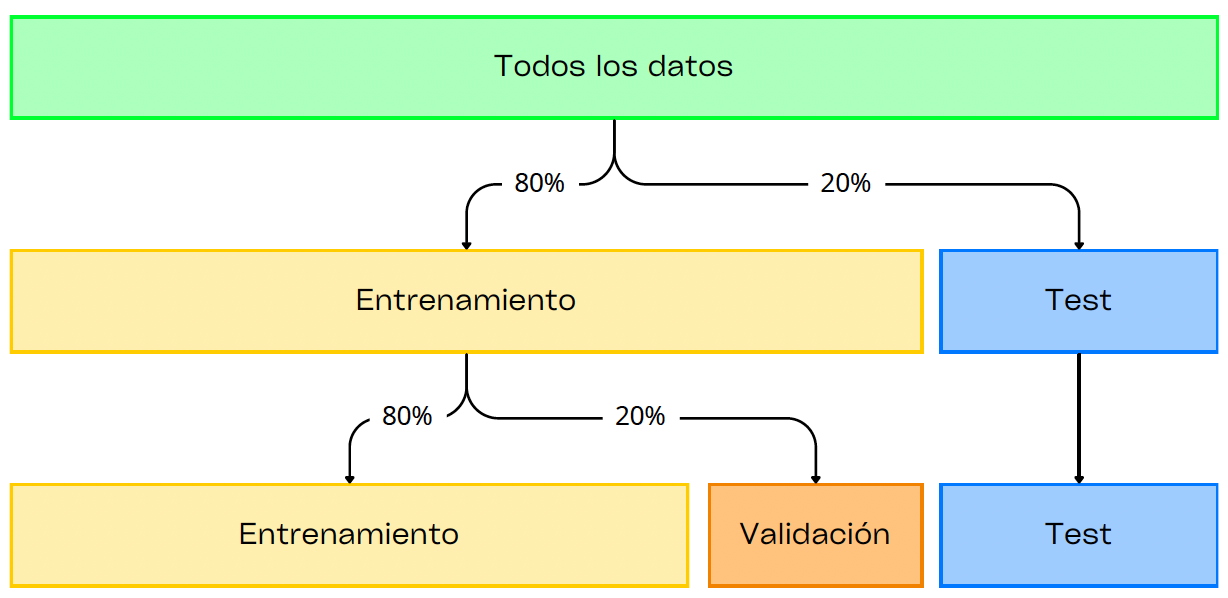
\includegraphics[scale=0.55]{imagenes/cap5/hold-out.png}
	\caption[Esquema de división del conjunto de datos.]{Esquema de división del conjunto de datos total en los subconjuntos de entrenamiento, validación y test.}
	\label{fig27}
\end{figure}

Considerando que el conjunto completo incluye los datos de los 4 modelos a utilizar (F27, F35, F53, F83.6), el primer paso consiste en reservar todas las imágenes de 30 sujetos de forma aleatoria para el conjunto de test. Posteriormente, se añaden imágenes adicionales de manera aleatoria, manteniendo las mismas distribuciones de focales, para constituir el 20\% del conjunto total de test, mientras que el 80\% restante se asigna al conjunto de entrenamiento.

Finalmente, durante el proceso de entrenamiento de los modelos, se aparta un 20\% aleatorio del conjunto de entrenamiento como conjunto de validación, dejando el 80\% restante para el entrenamiento propiamente dicho. Por tanto, para cada modelo focal contamos con 66528 imágenes, de las cuales 42577 se destinan al entrenamiento, 10645 a la validación y 13306 a test.

\subsection{Métricas}

Dado que se aborde un problema de regresión en el que la importancia de la distorsión en distancias cercanas es crucial, hemos optado por emplear la distorsión como función de pérdida. Esta medida se calcula mediante la siguiente fórmula:

\begin{equation}
	\text{Distorsion} = \displaystyle \frac{\sum_{i=1}^{n} | \displaystyle \frac{1}{1 + \displaystyle \frac{y_i}{d}} - \displaystyle \frac{1}{1 + \displaystyle \frac{x_i}{d}}|}{n}
\end{equation}

siendo $y_i$ la distancia verdadera en la imagen $i$, $x_i$ la distancia predicha en la imagen $i$, y $d = 12.6572 $ cm, que corresponde a un valor derivado de cálculos geométricos \cite{55} para obtener experimentalmente el factor de distorsión de una cabeza humana de tamaño promedio, según la SCD de la fotografía.

Esta función de pérdida asegura que el modelo aprenda a predecir distancias cercanas con mayor precisión, mitigando así la posibilidad de una distorsión significativa.

Aunque la distorsión se considera la medida principal de rendimiento, también se han empleado otras métricas como el error absoluto medio (MAE) y el error relativo medio (MRE) para evaluar el desempeño del modelo:

\begin{equation}
	\text{MAE} = \frac{1}{n} \sum_{i=1}^{n} | y_i - x_i |
\end{equation}

\begin{equation}
	\text{MRE} = \frac{1}{n} \sum_{i=1}^{n} \frac{| y_i - x_i |}{y_i}
\end{equation}

El MAE, al calcular la diferencia absoluta promedio entre las predicciones del modelo y los valores reales, mide cuánto se desvían las predicciones del modelo en términos absolutos. Esto es útil para entender la magnitud de los errores de predicción sin considerar su distorsión.
Por otro lado, el MRE, al calcular la diferencia relativa promedio entre las predicciones del modelo y los valores reales, proporciona una medida de cuánto se desvían las predicciones del modelo en relación con la distancia real (normalmente en porcentaje). Esto es fundamental cuando se necesita evaluar el rendimiento del modelo en términos de precisión relativa.


\subsection{Experimentos VGG16}
% En este apartado realizamos el entrenamiento de nuestros modelos con el nuevo dataset. Comparamos con los resultados de FacialSCDnet para ver si nuestro nuevo dataset mejora de algún modo el entrenamiento.

\subsubsection{Tuneo de hiperparámetros}

\subsubsection{VGG16}

% Además, en otro apartado se podrían utilizar otras arquitecturas distintas a VGG16 para comparar con esta.